\section{System architecture}

The proposed system consists of two major software components :
\begin{itemize}
\item
  ARTDAQ : handles the trigger farm and the data processing
\item
  MIDAS : handles the run configuration, run control, messaging,
  standardizes interfaces between various parts of the online system,
  and provides web-based interface for the shifters,
\end{itemize}

ARTDAQ supports computing farms with distributed architecture, 
and all high-bandwidth data traffic goes through ARTDAQ.

MIDAS architecture assumes a central server and multiple clients,
best suited for configuration/control applications.

The architecture of the proposed DAQ system is schematically presented
in Figure ~\ref{figure:system_architecture}.

\begin{figure}[H]
  \begin{tikzpicture}
    \node[anchor=south west,inner sep=0] at (0,0.) {
      % \node[shift={(0 cm,0.cm)},inner sep=0,rotate={90}] at (0,0) {}
      \makebox[\textwidth][c] {
        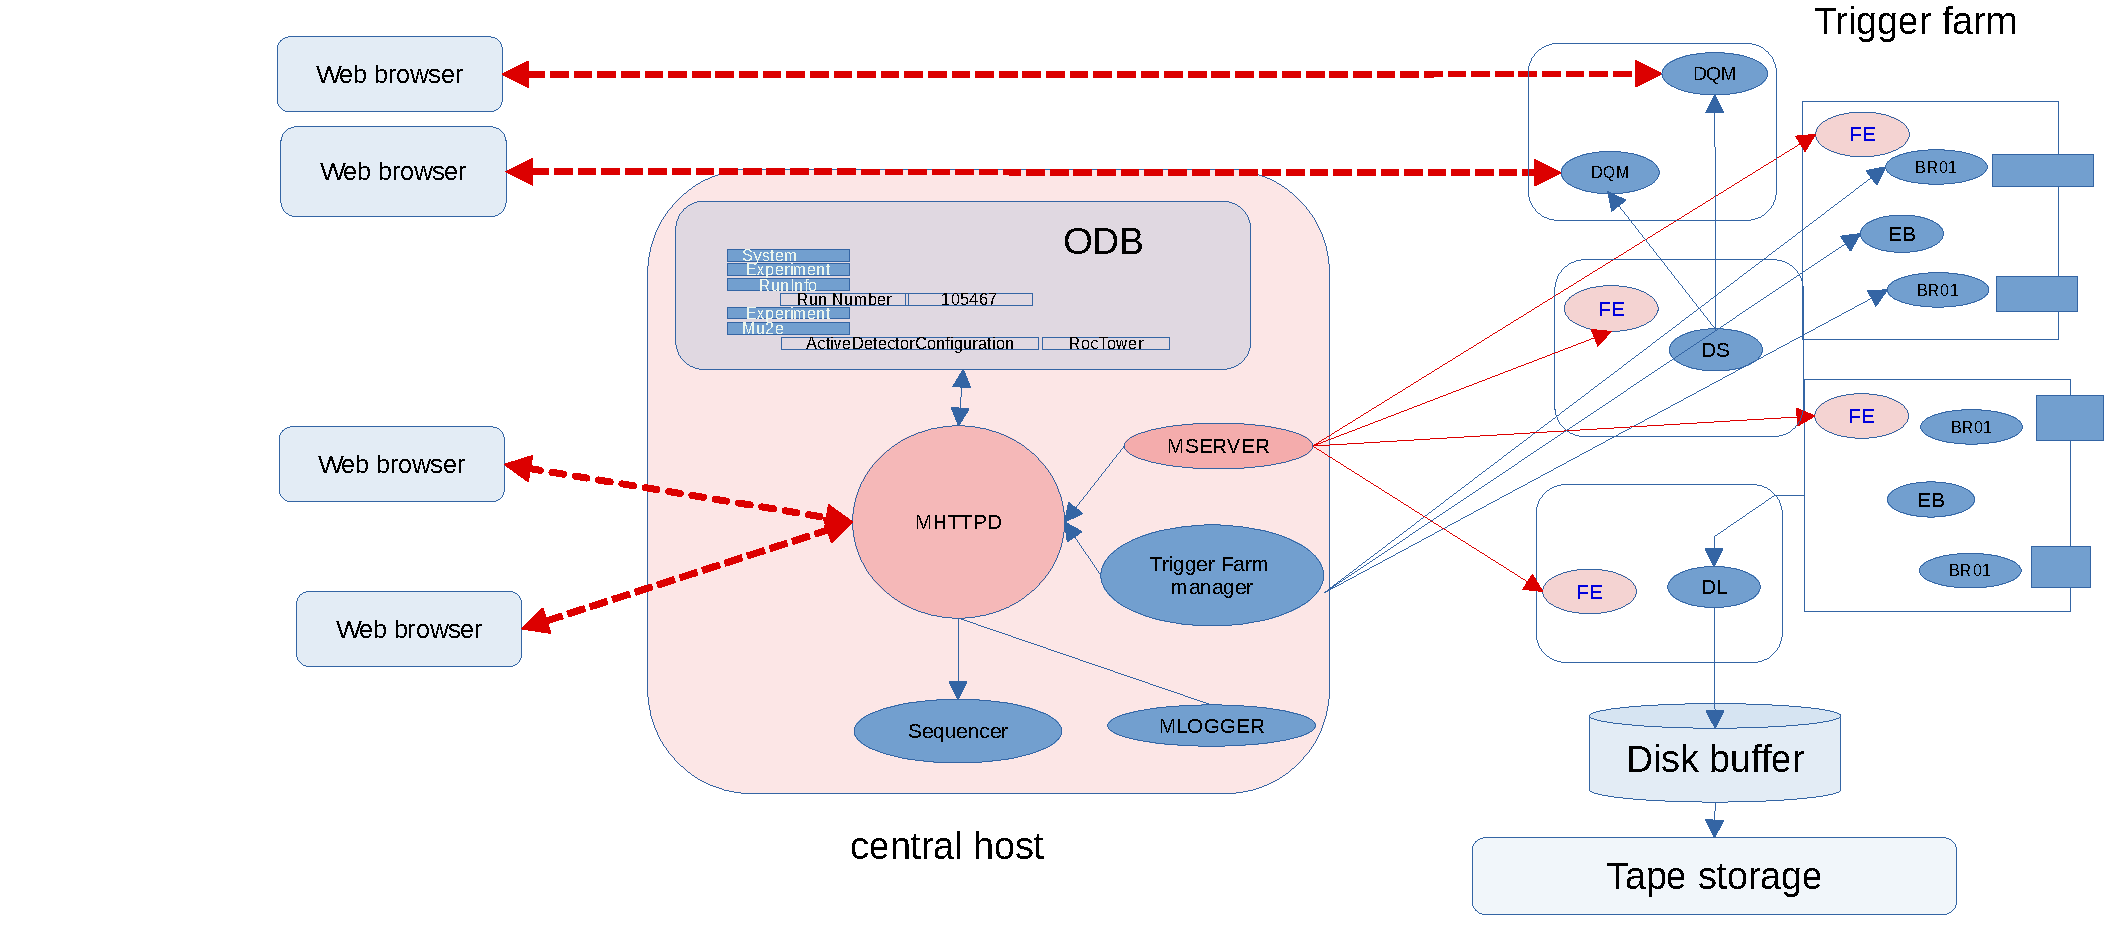
\includegraphics[width=1.1\textwidth]{pdf/system_architecture}
      }
    };
    % \node [text width=8cm, scale=1.0] at (14.5,0.5) {$\mu_B$, expected background mean};
    % \node [text width=8cm, scale=1.0, rotate={90}] at (1.5,7.5) { $S_{D}$, ``discovery'' signal strength  };
  \end{tikzpicture}
  \caption{
    \label{figure:system_architecture}
    Architecture of the MIDAS-based DAQ system. Communication protocols:
    red solid lines - JSON-RPC, blue solid lines - XML-RPC,
    red dashed lines - http(s).
  }
\end{figure}

%%%%%%%%%%%%%%%%%%%%%%%%%%%%%%%%%%%%%%%%%%%%%%%%%%%%%%%%%%%%%%%%%%%%%%%%%%%%%%
\subsection{MIDAS}

COre parts of MIDAS are :

\begin{itemize}
\item 
  mhttpd, a web server with restricted functionality
  mhttpd connects its clients to ODB. 
  The mhttpd doesn't execute any applications. Instead, it only updates the ODB.
\item
  Clients: frontends, communicating with the hardware and other
  parts of the system. Different types of frontends. Mu2e only needs slow monitoring.
\item
  Online DataBase (ODB) - a shared memory segment, which stores all configuration data of the system. Despite its name, ODB is not a database. Instead, it stores only current configuration
  of the system, As the new run starts, a run number-stamped configuration is exported and stored.
  Logical organization of ODB maps onto a json structure and is well suited for describing
  complex configurations with multiple levels of hierarchy
\end{itemize}

MIDAS ODB has several interfaces:
\begin{itemize}
\item 
  web-based interface - via the mhttpd ODB page
\item
  command line interface (odbedit)
\item
  C++ interface allowing C++ clients to interact with ODB
\item
  python interface
\end{itemize}

In all cases, clients connect to MHTTPD and MHTTPD acts as
the only agent directly interacting with the ODB.

%%%%%%%%%%%%%%%%%%%%%%%%%%%%%%%%%%%%%%%%%%%%%%%%%%%%%%%%%%%%%%%%%%%%%%%%%%%%%%
\subsection{Frontends}

MIDAS supports frontends of different types, which include the data readout and monitoring
frontends.

MIDAS event building functionality is not used , done by ARTDAQ.

The architecture of the Mu2e DAQ requires only monitoring and slow control frontends.


%%%%%%%%%%%%%%%%%%%%%%%%%%%%%%%%%%%%%%%%%%%%%%%%%%%%%%%%%%%%%%%%%%%%%%%%%%%%%%
\subsection{Interface to ARTDAQ}
All high bandwidth traffic goes through ARTDAQ.

ARTDAQ processes are controlled by the Trigger Farm Manager (TFM) frontend,
tfm\_launch\_fe.py.

\begin{itemize}
\item 
  TFM reads its initial settings from the "/Mu2e/ActiveRunConfiguration/DAQ/Tfm"
  ODB configuration path.
\item
  FCL files of ARTDAQ processes are stored in \$MU2E\_DAQ\_DIR/config/\$run\_configuration
  subdirectory assumed to be the same (network mounted) on all DAQ nodes.
  The FCL files could be regenerated manually based on the run configuration and the trigger table.
\item
  Archival mechanism: the FCL files used for a given run are stored
  in \$DAQ\_OUTPUT\_TOP/run\_records/\$run\_number area of the node where the TFM frontend is running.
\item
  the log files of ARTDAQ processes running on a given node are stored in \$DAQ\_OUTPUT\_TOP/logs
  directory of that node
\end{itemize}

%%%%%%%%%%%%%%%%%%%%%%%%%%%%%%%%%%%%%%%%%%%%%%%%%%%%%%%%%%%%%%%%%%%%%%%%%%%%%%
\subsubsection{Naming conventions for ARTDAQ components}

It is assumed that :
\begin{itemize}
\item 
  artdaq boardreaders described in the configuration have names "br01", "br02", etc
\item 
  artdaq event builders have names "eb01", "eb02", etc
\item 
  artdaq data loggers have names "dl01", "dl02", etc
\item 
  artdaq dispatchers have names "ds01", "ds02", etc
\end{itemize}

This convention allows to use component names, as they are, in the monitoring system.

%%%%%%%%%%%%%%%%%%%%%%%%%%%%%%%%%%%%%%%%%%%%%%%%%%%%%%%%%%%%%%%%%%%%%%%%%%%%%%
\subsubsection{Port assignment for ARTDAQ XML-RPC communication}
\begin{itemize}
\item
  base\_port: 10000+1000*partition\_number
\item 
  TFM : base\_port
\item 
  MIDAS node monitoring frontend: base\_port+11;
\item 
  artdaq boardreaders: base\_port+101 and base\_port+102
\item 
  artdaq event builders : base\_port + 201 - base\_port+300;
\item 
  artdaq data loggers  : base\_port + 301 - base\_port+400;
\item 
  artdaq dispatchers : base\_port + 401 - base\_port+500
\end{itemize}


%%%%%%%%%%%%%%%%%%%%%%%%%%%%%%%%%%%%%%%%%%%%%%%%%%%%%%%%%%%%%%%%%%%%%%%%%%%
\subsubsection{Communication with ARTRAQ}

\begin{itemize}
\item
  native artdaq communication is internal to the ARTDAQ
\item
  ARTDAQ processes report their metrics in XML-RPC format,
  and it is assumed that parsing of the metrics, visualizing
  it and generating alarms is the job of the 3-rd party application,
  i.e. {\bf grafana}.
\item
  TFM queries the ARTDAQ process metrics over XML-RPC and records
  them in ODB. That obsoletes the need in the 3rd party applications.
\item
  Mu2e -specific applications, i.e. the boardreaders and the filter modules 
  communicate to the MIDAS server directly via messaging and report 
  their status. Therefore simple alarms like single ROC timeouts etc
  could be generated as they are detected. 
  This avoids a need in an additional software to recognize an alarming
  situation and trigger the corresponding notification mechanism.
\end{itemize}


%%%%%%%%%%%%%%%%%%%%%%%%%%%%%%%%%%%%%%%%%%%%%%%%%%%%%%%%%%%%%%%%%%%%%%%%%%%%%%
\subsection{Interface to the online run conditions database} 

\begin{itemize}
\item
  the interface is provided by the MIDAS Sequencer and 
  \href{https://github.com/pavel1murat/frontends/blob/main/conf/mu2e_config_fe.py}
  {\blue the global configuration frontend}.
\item
  before the TFM starts, the configuration frontend requests a new run 
  number from the run configuration DB.
\item
  at begin run, the TFM frontend passes the run number to ARTDAQ processes.
\item
  the global configuration frontend registers the start and the stop of each
  run transition in the run configuration database.
\end{itemize}


%%%%%%%%%%%%%%%%%%%%%%%%%%%%%%%%%%%%%%%%%%%%%%%%%%%%%%%%%%%%%%%%%%%%%%%%%%%%%% 
\subsection{Slow monitoring and interface to EPICS}

The slow monitoring framework is provided by the MIDAS history system.
THis is one of the best technical solutions to the slow monitoring problem possible.
The interface via ODB is simple and crisp:
\begin{itemize}
\item
  all parameters to be monitored are stored by the monitoring frontends in ODB.
\item
  the visualization utilities simply display the content of the predefined ODB locations.
\end{itemize}

Therefore, the visualization and control is completely decoupled from the collection of the
monitoring parameters.

The historical data could be stored in  MIDAS internal format or in a database.
The list of supported databases includes ODBC, SQLITE, MYSQL and PGSQL.

This functionality is similar to that of grafana, however integrated with the
run control system

\begin{itemize}
\item
  one monitoring frontend per node 
  \begin{itemize}
  \item
    controls and configures DTC's and ROCs on this node
  \item
    controls the CFO if the CFO is running on this node
  \item
    monitors DTCs and ROCs, collecting history and non-history information
  \item
    monitors artdaq processes d separate collection of the monitoring information and its visualization
  \end{itemize}
\end{itemize}

Figure ~\ref{figure:slow_controls_node_page} gives an example of one of the slow controls pages

\begin{figure}[H]
  \begin{tikzpicture}
    \node[anchor=south west,inner sep=0] at (0,0.) {
      % \node[shift={(0 cm,0.cm)},inner sep=0,rotate={90}] at (0,0) {}
      \makebox[\textwidth][c] {
        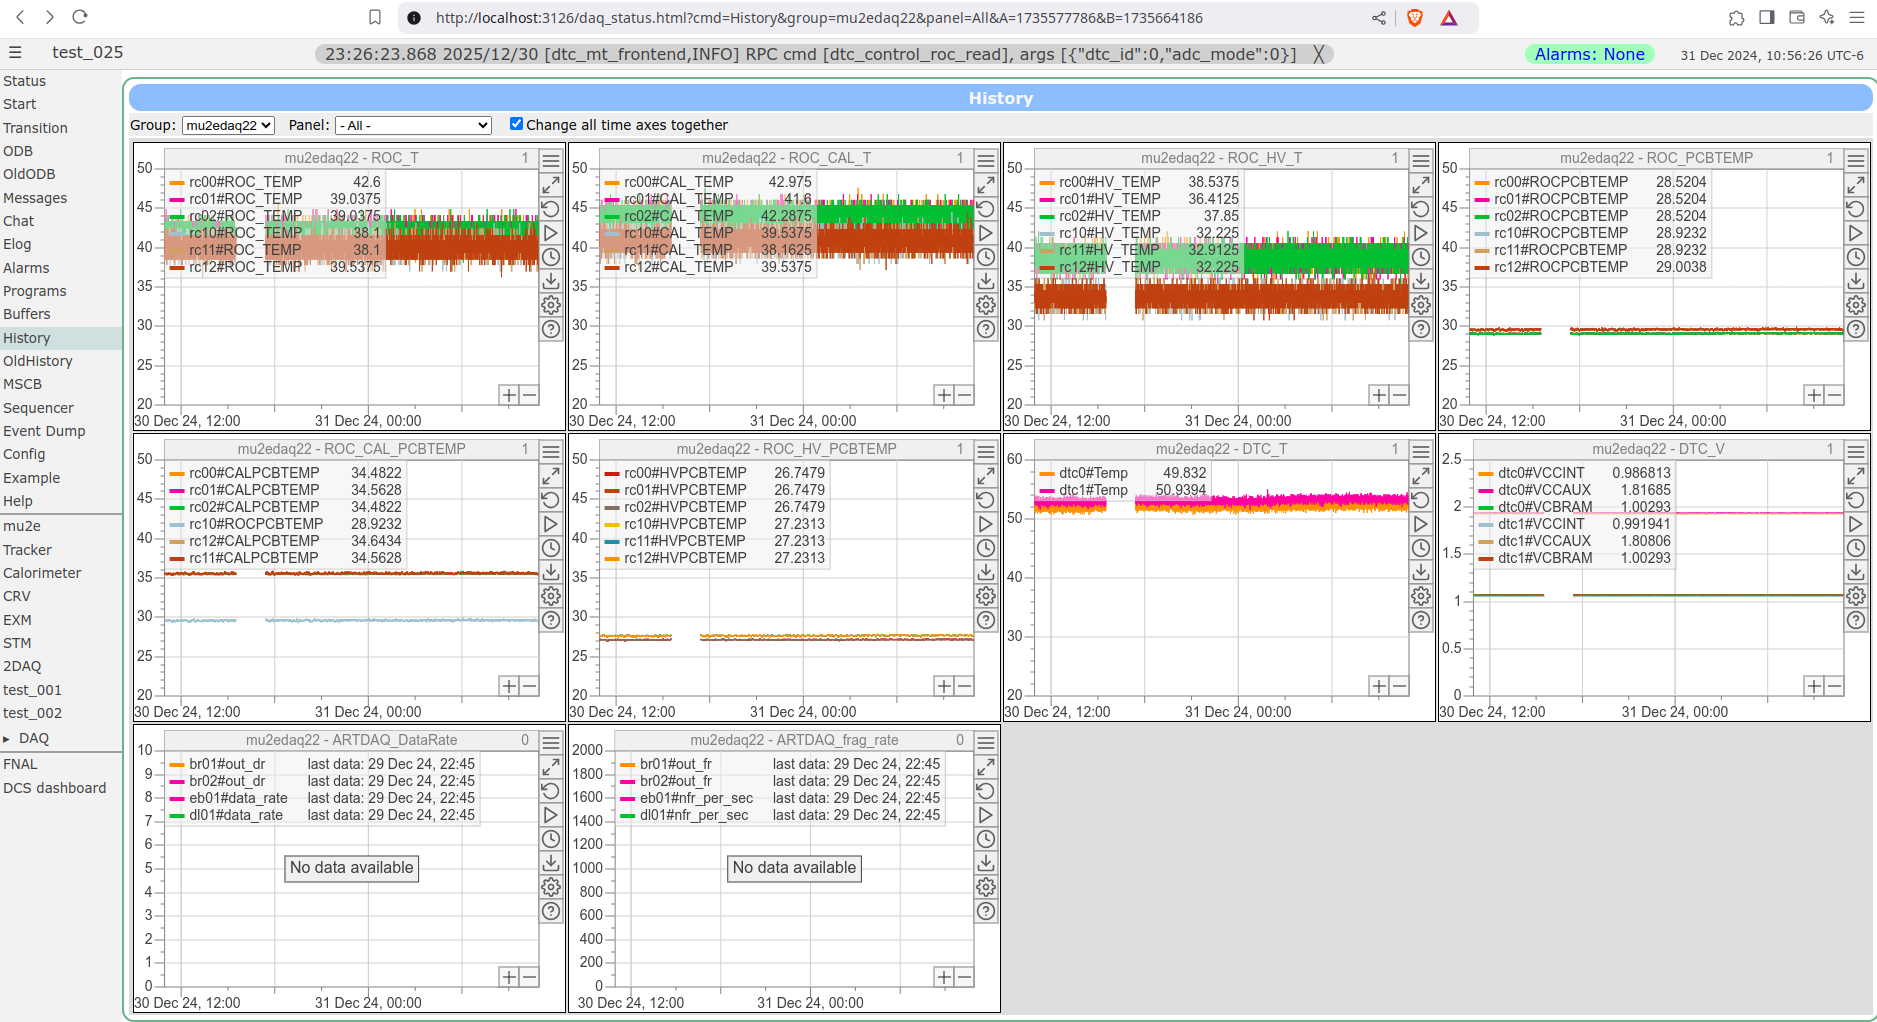
\includegraphics[width=0.95\textwidth]{png/slow_controls_node_page}
      }
    };
    % \node [text width=8cm, scale=1.0] at (14.5,0.5) {$\mu_B$, expected background mean};
    % \node [text width=8cm, scale=1.0, rotate={90}] at (1.5,7.5) { $S_{D}$, ``discovery'' signal strength  };
  \end{tikzpicture}
  \caption{
    \label{figure:slow_controls_node_page}
    A prototype of the DAQ node slow control page. Monitored are the DTC and ROC temperatures and voltages
    and rates of the ARTDAQ processes
  }
\end{figure}


In addition to its own fully implemented history system, MIDAS also has an interface to EPICS.
The interface is implemented as a 
\href{https://bitbucket.org/tmidas/midas/src/develop/examples/epics/}
         {\blue slow control frontend} with the 
\href{https://bitbucket.org/tmidas/midas/src/develop/drivers/device/epics_ca.cxx}
{\blue special EPICS driver}.
%
One therefore can in a transparent way combine EPICS data collection capabilities 
with the MIDAS web display system. MEG-II uses this approach for the beam parameter monitoring.

%%% Local Variables:
%%% mode: latex
%%% TeX-master: t
%%% End:


%%%%%%%%%%%%%%%%%%%%%%%%%%%%%%%%%%%%%%%%%%%%%%%%%%%%%%%%%%%%%%%%%%%%%%%%%%%%%%
\subsection{Alarm system}

MIDAS has a built-in alarm system which could be used to inform shifters
about various categories of failures.

That is not a replacement for critical alarms coming from different inputs.
CRYO ? Accelerator ? -{\red talk to Andy Hocker.}


%%%%%%%%%%%%%%%%%%%%%%%%%%%%%%%%%%%%%%%%%%%%%%%%%%%%%%%%%%%%%%%%%%%%%%%%%%%%%% 
\subsection{Javascript web interface}

\begin{itemize}
\item 
  MIDAS web interface is a combination of HTML5+Javascript, based on the
  asynchronous approach to the web pages update (Ajax).
\item 
  MIDAS provides Javascript API to ODB, which facilitates development of
  functional experiment-specific {\bf custom} web pages.
  The interface is documented at \\
  \href{https://daq00.triumf.ca/MidasWiki/index.php/Custom\_Page}
  {\blue https://daq00.triumf.ca/MidasWiki/index.php/Custom\_Page}
\end{itemize}


%%%%%%%%%%%%%%%%%%%%%%%%%%%%%%%%%%%%%%%%%%%%%%%%%%%%%%%%%%%%%%%%%%%%%%%%%%%%%%
\subsection{Interfaces to ECL, ELOG, Slack}

MIDAS has interfaces to internal and external ELOGs and Slack.
\begin{itemize}
\item
  interface to the external ELOG has been implemented and tested
\item
  interface to Slack has been tested and used by at least two experiments - MEG and g-2
\item
  interface to ECL - to be implemented
\end{itemize}


%%%%%%%%%%%%%%%%%%%%%%%%%%%%%%%%%%%%%%%%%%%%%%%%%%%%%%%%%%%%%%%%%%%%%%%%%%%%%%
\subsection{DQM}

DQM processes use ROOT-based histogramming. As any ROOT executable is a web server,
the DAQM jobs publish their histograms on the web, and their clients (users)
simply connect to them over the http protocol.

%%%%%%%%%%%%%%%%%%%%%%%%%%%%%%%%%%%%%%%%%%%%%%%%%%%%%%%%%%%%%%%%%%%%%%%%%%%%%% 
\subsection{Interprocess communication} 

The system supports three mechanisms
\begin{itemize}
\item
  via ODB : some clients write into ODB, others read
\item
  separate collection of the monitoring information and its visualization
\item
  MIDAS messaging: jsonrpc.
  \begin{itemize}
  \item
    Each client can have a jsonrpc server and receive messages
    from any other client.
  \item
    clients can broadcast messages to the system (info and alarm)
    and communicate to each other
  \item
    each frontend, C++ or Python, has a built-in jsonrpc communication
    functionality built-in.
  \end{itemize}
\item
  communication between ARTDAQ processes is based on an older technology,
  XML-RPC. The TFM frontend supports the XML-RPC-based ARTDAQ communication
  protocol.
\end{itemize}
